\documentclass{article}

\usepackage[utf8]{inputenc}

%\usepackage{natbib}
\usepackage{hyperref}

\usepackage{graphicx}

\usepackage[colorinlistoftodos]{todonotes}

\usepackage{parskip}
\setlength{\parskip}{10pt} 

\usepackage{tikz}
\usetikzlibrary{arrows, decorations.markings}

\usepackage{outlines}

\usepackage{chngcntr}
\counterwithout{figure}{section}

\usepackage{pgfgantt}



\begin{document}


\begin{titlepage}
  

\centering
  
  
{\scshape\LARGE Master thesis Planning Report\\}
  
\vspace{0.5cm}
  
{\huge\bfseries Injection of Information to Embodied Agents\\}

  
\vspace{2cm}
  
{\Large Yasmeen Emampoor (gusemampya@student.gu.se)\\}
  
\vspace{1.0cm}
  
{\large Supervisor: Simon Dobnik (FLoV)\\}
  
\vspace{1.5cm}

\end{titlepage}
  
\section{Introduction}
\subsection{Background}
Robots are able to perform tasks that are tedious or even dangerous for humans, giving them the potential to be useful in a variety of fields. Robots working within human areas are often operated based on pre-defined actions, or remotely. Being able to give a robot instructions and interact with it in natural language would allow for increased efficiency. \\
One example of this would be with household agents, which move within a home and help carry out tasks. An average user is unlikely to be a robotics expert, and so being able to interact with the agent in a similar way to how one would with another person would be ideal.

\begin{verbatim}
Human: Go get my computer from the office. 
Robot navigates to the office, finds the computer, brings it back. 
Human: Were my keys in the office?
Robot: I don't know, I'll go check. 
Robot navigates to the office, finds the keys. Returns.
Robot: Yes, they are on the bookshelf. 
Human: Thanks. 
\end{verbatim}
For this project, I'm considering a simpler dialogue stub: the human asks a question, and the robot answers. 
\begin{verbatim}
Q: Where is the computer?
A: In the office. 
\end{verbatim}

\subsection{Aim}
The task in which an embodied agent is asked a question and must move within its surroundings in order to answer it is called Embodied Question Answering (EQA). EQA is essentially a combination of two tasks, navigation and Visual Question Answering (VQA).\\
The aim of this thesis is to identify ways in which prior or extra knowledge can be used to improve model performance in an EQA task. 

Hypotheses: 
\begin{outline}
	\1 The VQA model does consider the visual features when answering the questions.
		\2 If true, additional view points can improve performance in the VQA task. 
	\1 Transfer learning to incorporate pre-trained features in feature extraction can improve performance on both the VQA and Navigation tasks.
\end{outline}


\subsection{Limitations}
The dataset of questions and answers for EQA in Habitat was automatically generated, and may contain some errors. One example of this is shown in Fig.~\ref{fig:err_ex}, in which a VQA model answered that the sofa in the living room is tan, but the ground truth answer is that it is yellow. However, looking at the image, I see a tan sofa and a yellow armchair. It seems that an error was likely made in the automatic question/answer generation, identifying the armchair as a sofa, but the model is not making the same error. \\
\begin{figure}[h]
	\centering
	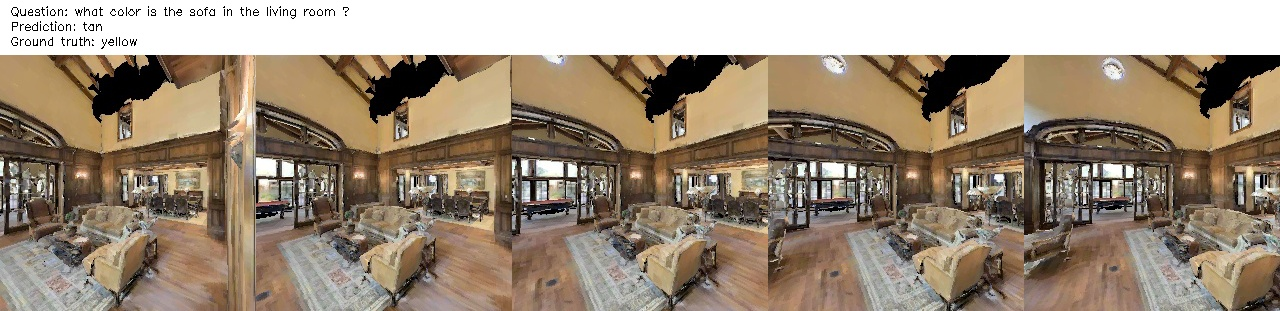
\includegraphics[width=\textwidth]{../error_images/ckpt_0_121_image.jpg}
	\caption{Error Example}
	\label{fig:err_ex}
\end{figure}
Certain colors, such as brown, are also over represented in the dataset. However, I plan to work with this dataset as is, rather than attempting to balance presence of colors, or manually removing incorrect question answer pairs. This is both due to time limitations, and due to not wanting to introduce artificial balance--many things in houses are made of wood, and are therefore brown. It's not necessarily a bad thing for the system to expect tables to be brown, as long as it is also actually looking for a table to answer the question. \\
A dataset was collected using humans via Amazon Mechanical Turk, but it relies on a house dataset that is no longer available. \\
\todo{classification vs generation}
 

\section{Methodology}
I am working with AI Habitat, a simulation platform for working with embodied AI\cite{habitat19iccv}. It consists of two parts, Habitat-Sim, the 3D simulator, and Habitat-Lab, the library for embodied AI development. I am using the Matterport3D dataset, a dataset of real interiors with human annotation of objects, as my scene dataset\cite{matterport}. \\
I am starting with the Embodied Question Answering baseline in Habitat-Lab, which consists of three parts, a CNN for initial feature extraction, a question answering module, and a navigation module, called Pacman\cite{embodiedqa}. I am using the EQA task dataset, which was created using code to automatically generate questions and answers to correspond with scenes in the Matterport3D dataset\cite{eqa_matterport}. \\
I am working in a GPU cluster through mlt, but also am going to create a mini-version of the dataset that I can use to run tests locally, although fully training or evaluating will need to happen on a GPU, due to the size of the dataset. \\
I will be considering two metrics for the VQA task: mean rank and accuracy. For the navigation task, I will consider the percentage of questions in which the agent ended in the room containing the target. \\
The first task is to determine if the VQA model is considering the visual input when answering the questions. To do this, I will run evaluation normally, where the VQA model gets the images, and "blindfolded", where the VQA does not. To do this, I have duplicated a method that converts the images to an array to input to the model, and modified it to produce an array of zeros instead. Preliminary results with this suggest that the VQA model is considering the visual features--it performs worse on evaluation when blindfolded. This is interesting, because another student performed a similar test in a course project, where they gave the VQA wrong images, and they did not see decrease in performance. I plan to implement that method of blindfolding as well, and compare the results between the two methods. \\
Assuming that the model is considering visual input, the next step is to give the model more variety in the viewpoints it is considering, since the shortest path navigation being learned may not give the best views for answering the question\cite{blindfolded}. I plan to do this by implementing a look-around procedure for the agent to do at the end of each shortest path navigation. Custom actions can be defined in habitat, so I plan to implement special turning actions with larger movement than the standard actions, and then have the agent perform these at the end of each navigation during training. The limited views of the shortest path can be seen in Fig.~\ref{fig:viewpoints}, which shows the last five steps the agent took.

\begin{figure}[h]
	\centering
	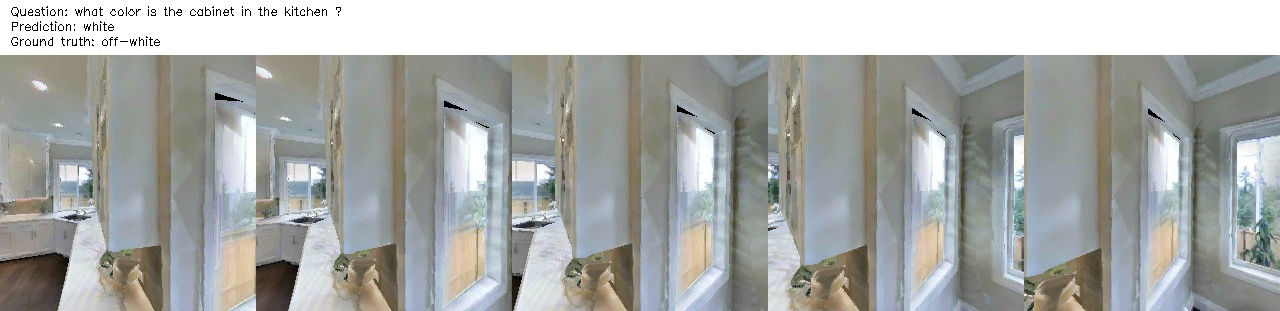
\includegraphics[width=\textwidth]{ckpt_0_1093_image.jpg}
	\caption{Limited Viewpoints}
	\label{fig:viewpoints}
\end{figure}

The next task is to incorporate pre-training in the CNN, to test if this improves performance, both in the VQA task, and in the navigation task, both of which rely on the same CNN for feature extraction and segmentation. My current plan for this is to stack the current CNN on a pretrained network like vgg19, but this may change. \\
There is also a semantic sensor within habitat that could be enabled for the VQA and navigation tasks, which reads semantic annotations from the simulated scene. One concern with this is that it might simply make up for weaknesses in the CNN, which is meant to be doing segmentation. 

\section{Schedule}
\begin{ganttchart}[
	hgrid=true,
	vgrid=true,
	bar/.append style={fill=gray},
	canvas/.append style={fill=none},
	link/.append style={thick}
	]{1}{17}
	\gantttitle{Schedule}{17} \\
	\gantttitlelist{5, ..., 21}{1} \\
	\ganttbar{Getting GPU Access}{2}{2} \\
	\ganttbar{Attend presentation on blindfolding}{2}{2} \\
	\ganttbar{Learning Habitat}{1}{6} \\
	\ganttbar{Writing Seminar I}{2}{2} \\
	\ganttbar{Train\&Eval.Baseline, blindfolded\&normal}{6}{7} \\
	\ganttbar{Make Mini-Dataset}{7}{7} \\
	\ganttbar{Implement Look Around}{8}{9} \\
	\ganttbar{Incorporate pre-training in the CNN}{9}{11} \\
	\ganttbar[bar/.append style={fill=red}]{GPU Off}{8}{8} \\
	\ganttbar[bar/.append style={fill=cyan}]{Writing Seminar II}{12}{14} \\
	\ganttbar{Writing!}{14}{16} \\
	\begin{scope}[on background layer]
	\ganttlink{elem0}{elem4}
	\ganttlink{elem4}{elem6}
	\ganttlink{elem4}{elem7}
	\end{scope}
\end{ganttchart}
\todo{presentation dates?}


\section{Risk Analysis and Ethical Considerations}
The main risks to completion of this project are related to running out of time--habitat is a new environment for me to work in, so unexpected difficulties are likely to pop up, and the data is too large to work locally, but there are always risks to working on shared servers--at the moment some of the GPUs in the cluster I am using are behaving strangely, and although the issue is under investigation, it is slowing down some of the work. \\
An important note ethically is that the original development of this model, not the version included in Habitat-Lab, but the original version associated with the EmbodiedQA project, was developed using a dataset that, as of July 2020, was the subject of a lawsuit by the company Planner5D against Facebook and Princeton, on the grounds that the data was accessed without permission\cite{planner5d}. This is not the dataset that I will be using, but it was used in the development of the baseline and the development of the Embodied Question Answering task definition. 


\bibliographystyle{ieeetr}
\bibliography{references}

\end{document}

